%Authors guidlines: http://royalsocietypublishing.org/instructions-authors#question5

\documentclass[12pt,letterpaper]{article}
\usepackage{natbib}

%Packages
\usepackage{pdflscape}
\usepackage{fixltx2e}
\usepackage{textcomp}
\usepackage{fullpage}
%\usepackage{natbib}
\usepackage{float}
\usepackage{latexsym}
\usepackage{url}
\usepackage{epsfig}
\usepackage{graphicx}
\usepackage{amssymb}
\usepackage{amsmath}
\usepackage{bm}
\usepackage{array}
\usepackage[version=3]{mhchem}
\usepackage{ifthen}
\usepackage{caption}
\usepackage{hyperref}
\usepackage{amsthm}
\usepackage{amstext}
\usepackage{enumerate}
\usepackage[osf]{mathpazo}
\usepackage{dcolumn}
\usepackage{lineno}
\usepackage{longtable}
\pagenumbering{arabic}


%Pagination style and stuff
\linespread{2}
\raggedright
\setlength{\parindent}{0.5in}
\setcounter{secnumdepth}{0} 
\renewcommand{\section}[1]{%
\bigskip
\begin{center}
\begin{Large}
\normalfont\scshape #1
\medskip
\end{Large}
\end{center}}
\renewcommand{\subsection}[1]{%
\bigskip
\begin{center}
\begin{large}
\normalfont\itshape #1
\end{large}
\end{center}}
\renewcommand{\subsubsection}[1]{%
\vspace{2ex}
\noindent
\textit{#1.}---}
\renewcommand{\tableofcontents}{}
%\bibpunct{(}{)}{;}{a}{}{,}

%---------------------------------------------
%
%       START
%
%---------------------------------------------

\begin{document}

%Running head
\begin{flushright}
Version dated: \today
\end{flushright}
\bigskip
\noindent RH: Morphological data availability in living mammals

\bigskip
\medskip
\begin{center}

\noindent{\Large \bf Morphological data availability in living mammals}
%Or: Missing morphological data in living mammals - but I prefer the first one emphasizing on the availability of it. The data is not missing per se, it's just not coded!

%Key words: Total Evidence method, data structure, phylogenetic, living, fossil, topology
\bigskip

\noindent {\normalsize \sc Thomas Guillerme$^1$$^,$$^2$$^*$, and Natalie Cooper$^1$$^,$$^2$}\\
\noindent {\small \it 
$^1$School of Natural Sciences, Trinity College Dublin, Dublin 2, Ireland.\\
$^2$Trinity Centre for Biodiversity Research, Trinity College Dublin, Dublin 2, Ireland.}\\
\end{center}
\medskip
\noindent{*\bf Corresponding author.} \textit{Zoology Building, Trinity College Dublin, Dublin 2, Ireland; E-mail: guillert@tcd.ie; Fax: +353 1 6778094; Tel: +353 1 896 2571.}\\
\vspace{1in}

%Line numbering
%\modulolinenumbers[1]
%\linenumbers

%---------------------------------------------
%
%       ABSTRACT
%
%---------------------------------------------

\newpage
\begin{abstract}
Studying changes in global biodiversity through time and space is essential.
For that we need methods to combine both palaeontological and neontological data.
One promising method, the Total Evidence method, allows such thing but needs a lot of data.
Especially morphological data from living taxa to allow the fossil taxa to accurately branch in the trees.
Despite two centuries of morphological studies on living taxa, scientists using and generating such data mainly focus on palaeontological data.
Therefore, even in well known groups such as mammal, there is a huge gap in our knowledge of morphological data for living mammals.
In this study, using phylogenetic community structure methods, we quantify the availability of data in each mammalian order.
And maybe at the end of the paper we propose some discussion on how to improve all that (go in museums!).
\end{abstract}

\noindent ()\\

\vspace{1.5in}

\newpage 

%---------------------------------------------
%
%       INTRODUCTION
%
%---------------------------------------------

\section{Introduction}
%We need fossils - dangerously paraphrased from the missing data paper
Studying both living and fossil taxa together in essential to fully understand macrovelutionary patterns and processes and is becoming increasingly common among evolutionary biologists \citep{jacksonwhat2006,quentaldiversity2010,dietlconservation2011,slaterunifying2013,fritzdiversity2013,Wood01032013}. Combining the global biodiversity by including both living and fossil in such studies allows, for example, to improve accuracy of the timing of diversification events \citep[e.g.][]{ronquista2012}, to better understand relationships among lineages \citep[e.g.][]{beckancient2014} or to infer biogeographical patterns through time \citep[e.g.][]{Meseguer01032015}. %And add STD paper? Or that's too much self cites?
%We can use TEM for that
In order to perform such analysis, one must efficiently combine living and fossil taxa data in macroevolutionary models. One trending method, called the Total Evidence method \citep{eernissetaxonomic1993,ronquista2012}, allows to combine molecular data from living taxa and morphological data from both living and fossil taxa in a supermatrix \citep[e.g.][]{pyrondivergence2011,ronquista2012,schragocombining2013,slaterunifying2013,beckancient2014,Meseguer01032015}. This method not only allows to use all the available data but also allows to treat fossil taxa as tips rather than nodes \textit{via} integrative phylogenetic inference methods such as tip-dating \citep{ronquista2012,Drummond01082012,Wood01032013,BEASTmaster}.

%But missing data in living taxa problem
However, the Total Evidence method requires, by definition, a lot of data. One must collect both molecular data for living taxa as well as morphological data for both living and fossil taxa, two types of data that require fairly different technical skills \citep[e.g.][]{meredithimpacts2011} \textit{vs.} \citep{O'Leary08022013}. Additionally, entire sections of this data can sometimes be difficult or impossible to collect for every taxa present in the analysis. For example, fossil have really rarely molecular data available and morphological characters are rarely collected for living taxa when molecular data is available \citep[e.g.][]{slaterphylogenetic2013,beckancient2014}. This difference between both data can lead to topological errors in phylogenetic inference \citep{GuillermeCooper}. In fact, the ability of the Total Evidence method to recover correct topology is expected to decrease when there is a low overlap between morphological data from the living and the fossil taxa \citep{GuillermeCooper}. The effect of missing data is most important on topology when too few living taxa have available morphological data \citep{GuillermeCooper}. For example, if there is no morphological available for any living taxa within an entire clade, it is impossible to link a fossil taxon to this clade because no morphological data will overlap between the fossil (regardless the amount of data available for the fossil) and the living taxa (that have no morphological data). This property of the Total Evidence method can rapidly lead to important topological incongruities because the fossil will only be able to branch to a clade of living taxa that contains morphological data, even if in reality, the fossil taxon does not belong to that clade \citep{GuillermeCooper} (see figure ~\ref{Figure_missing_data_problem}.

\begin{figure}[!htbp]
\centering
    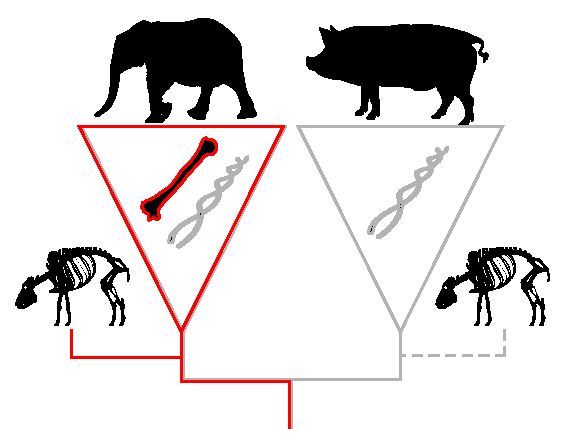
\includegraphics[width=1\textwidth]{MissingDataFigure.pdf}
\caption{Example of topological errors due to missing morphological data in living taxa. If a phylogeny contains two clades, for example Aves and Mammalia, with molecular data (in grey) for both but only morphological data (in red) for Aves. If an additional Mammalia fossil (with no molecular data) is added to the phylogeny, it will erroneously branch with the Aves clade instead of the Mammalia one because no morphological data will overlap between the fossil Mammalia and the living ones.}
\label{Figure_missing_data_problem}
\end{figure}

%What we're doing
It is therefore crucial to understand the distribution of the available morphological data for living taxa in a clade before using a Total Evidence approach because missing living taxa with morphological data can lead to two topological artefacts: (1) the impossibility for a fossil to branch in the right clade if there is no morphological data available in this clade \citep{GuillermeCooper}; and (2) the higher probability for a fossil to branch within a wrong clade that has more morphological data available for living taxa than the right clade \citep{GuillermeCooper}. In this study, we assess the level of available morphological data in living mammals in order to highlight the two caveats described above.
%In this study we investigate the amount of living mammal taxa with available morphological data to detect the two potential caveats described above that could lead to topological errors when building Total Evidence mammal phylogenetic trees.
We collected living mammals morphological data from @256 phylogenetic matrices available online and measured the proportion of morphological data availability for each mammalian order. Additionally, in the mammalian orders where data was missing, we estimated the structure of the available data to detect if the available data was biased towards certain clades only or if it was randomly distributed using the Net Relatedness Index \citep{webb2002phylogenies}.

%---------------------------------------------
%
%       METHODS
%
%---------------------------------------------
 
%\newpage

\section{Material and Methods}
\subsection{Matrices search}
To investigate the available living taxa with morphological data, we downloaded morphological matrices from three main public databases: morphobank (\texttt{http://www.morphobank.org/} \citep{morphobank}, Graeme Lloyd's website (\texttt{http://graemetlloyd.com/} and Ross Mounce's GitHub repository (\texttt{https://github.com/rossmounce}. We downloaded all the matrices containing any fossil or living mammal taxa from these databases. Additionally we ran a thorough Google Scholar search for matrices that might not have been uploaded on the previously cited data bases. We downloaded the additional morphological characters matrices from the 20 first Google search results matching with our selected keywords and with any of the 35 taxonomic levels (see supplementary materials for detailed description of the procedure). We downloaded 256 % @@@ Number of matrices
matrices containing a total of 9411 % @@@ Number of living OTUs
operational taxonomic units (OTUs) from the combination of both searches (public repositories and Google Scholar). The list of matrices is available in the supplementary materials.

We then transformed all the matrices to be in the same nexus format. We also standardised the taxonomic nomenclature by fixing invalid binomial inputs to match with the official taxonomic nomenclature rules (i.e. \textit{H. sapiens} was transformed in \textit{Homo sapiens}. We assigned each species as being either living or fossil using a taxonomic matching algorithm. We designated as living OTU all the OTUs that where either present in \citep{FritzTree} or \citep{wilson2005mammal}. We designated as fossil OTUs all the OTUs that where present in the Paleobiology database. For the OTUs neither labelled as living or fossil we tried to decompose the OTUs name (i.e. \textit{Homo$\_$sapiens} became \textit{Homo} and \textit{sapiens} and tried to match the first element with any taxonomic level (Family, Genus, Species, etc.) from \citep{wilson2005mammal}. The matching OTUs where labelled as living and the ones still not matching where ignored and labelled as non-applicable (NA; see supplementary material for more details on the taxonomic matching algorithm).

\subsection{Data availability analysis}
\subsubsection{Number of characters threshold}
From all the 256 % @@@ Number of matrices
matrices, we selected only the ones that displayed at least 100 morphological characters per OTU. This arbitrary threshold of a minimal number of morphological characters was chosen to be in adequacy with \citep{GuillermeCooper} and \citep{harrisonamong-character2014}. Also this threshold avoids biases towards small matrices that could be either not informative \citep{wagner2000} (e.g. too few characters not allowing character overlap among matrices) or made of non-applicable characters \citep{Brazeau2011} (e.g. antlers which are sexual dimorphic characters proper to a specific clade).

\subsubsection{Data availability}
To assess the data availability per mammal order, we calculated the percentage of OTUs with morphological data for three different taxonomic levels: Family, Genus and Species. We highlighted all the orders containing less than 25\% of living taxa with morphological data because their amount of missing data ($>$75\%) was higher than in \citep{GuillermeCooper} and therefore highly probable of having wrong topology due to the missing data. On the opposite, orders with up to 25\% of missing data (75\% of available data) were shown to have no significant effect on topology \citep{GuillermeCooper}. We therefore used this value as a threshold of "good" data sampling. 

\subsubsection{Available data structure}
For the orders with no morphological data for all its OTUs at the three different taxonomic levels (Family, Genus and Species), we investigated the structure of the available data to test if it was either (i) randomly distributed, (ii) over-dispersed or (iii) clustered. To measure the structure of the available data we used classic community structure metric from the \texttt{picante} R package \citep{picante}. We compared the structure of the available data for each order to the structure of a potentially fully sampled order (i.e. only the OTUs with available morphological data \textit{versus} all the OTUs).
For each orders and taxonomic levels that presented OTUs with no available morphological data, we calculated the Net Relatedness Index (NRI) which quantifies the overall distribution of the data with negative values showing more dispersed data and positive values more clustered data than expected by the null model (random) \citep{webb2002phylogenies}. We choose to present only the NRI values because they have been shown to be slightly less sensitive to the structure of the phylogeny (i.e. branch length and topology) \citep{NRI,journal.pone.0004390} but we also calculated the two other common phylogenetic structure indices: Faith's Phylogenetic Distance (PD) \citep{Faith19921} and the Nearest Taxon Index (NTI) \citep{webb2002phylogenies}. Both metrics are available in the Supplementary results.

%\subsubsection{Data improvement strategy}
%Phylotargeting
%This part as not been done at all! I was looking for a non-GUI version of Arnold and Nunn's software but there is none (Arnold confirmed by email). Therefore because I was focusing on the part above and to make it repeatable I didn't did that part yet. However, I still planing on doing it! I just need to find a bit of time to write some code to make it non-GUI (and to be able to use big trees).

All the following procedure is repeatable and available on GitHub. %Or what is the right way to show it's reproducible?

%---------------------------------------------
%
%       RESULTS
%
%---------------------------------------------

\section{Results}

\subsection{Data availability}
We extracted 1422 living mammal OTUs from the 256 matrices with a minimum of 6 characters and a maximum of 4541 per OTU. After removing all the matrices with less than 100 morphological characters, the number of extracted living mammals OTUs was down to 815. 11/28 orders have less than 25\% of taxa with morphological data at a species level and 24/28 orders have less than 75\% taxa with available morphological data. At the Genus level however only 3/28 orders have less than 25\% of taxa with morphological data and 16/28 have less than 75\%. Finally, at the family level no order has less than 25\% taxa with available morphological data and only 5/28 have less than 75\% (table \ref{Table_morpho_taxa_proportion}.

\renewcommand\baselinestretch{1.2}\selectfont
\begin{center}
% latex table generated in R 3.1.1 by xtable 1.7-3 package
% Fri Feb 27 10:08:44 2015
\begin{longtable}{llll}
\caption{Proportion of available OTUs with morphological data per order and per taxonomic level. We highlighted in bold the orders that have more than 75\% of missing data for each taxonomic level. Note that it is possible that more data is available at a higher taxonomic level (Genus $>$ Species) since if the species name for an OTU was not or miss specified, we still counted the OTU for higher taxonomic level analysis.} \\ 
  \hline
Order & Taxonomic level & Fraction of OTUs & Percentage of OTUs \\ 
  \hline
Monotremata & Family & 2/2 & 100 \\ 
  Monotremata & Genus & 2/3 & 66.67 \\ 
  Monotremata & Species & 2/4 & 50 \\ 
  Didelphimorphia & Family & 1/1 & 100 \\ 
  Didelphimorphia & Genus & 16/16 & 100 \\ 
  Didelphimorphia & Species & 40/84 & 47.62 \\ 
  Paucituberculata & Family & 1/1 & 100 \\ 
  Paucituberculata & Genus & 2/3 & 66.67 \\ 
  Paucituberculata & Species & 2/5 & 40 \\ 
  Microbiotheria & Family & 1/1 & 100 \\ 
  Microbiotheria & Genus & 1/1 & 100 \\ 
  Microbiotheria & Species & 1/1 & 100 \\ 
  Notoryctemorphia & Family & 1/1 & 100 \\ 
  Notoryctemorphia & Genus & 1/1 & 100 \\ 
  \textbf{Notoryctemorphia} & \textbf{Species} & \textbf{0/2} & \textbf{0} \\ 
  Dasyuromorphia & Family & 2/2 & 100 \\ 
  Dasyuromorphia & Genus & 7/22 & 31.82 \\ 
  \textbf{Dasyuromorphia} & \textbf{Species} & \textbf{8/64} & \textbf{12.5} \\ 
  Peramelemorphia & Family & 2/2 & 100 \\ 
  Peramelemorphia & Genus & 7/7 & 100 \\ 
  Peramelemorphia & Species & 16/18 & 88.89 \\ 
  Diprotodontia & Family & 9/11 & 81.82 \\ 
  Diprotodontia & Genus & 20/38 & 52.63 \\ 
  \textbf{Diprotodontia} & \textbf{Species} & \textbf{16/126} & \textbf{12.7} \\ 
  Afrosoricida & Family & 2/2 & 100 \\ 
  Afrosoricida & Genus & 17/17 & 100 \\ 
  Afrosoricida & Species & 23/42 & 54.76 \\ 
  Macroscelidea & Family & 1/1 & 100 \\ 
  Macroscelidea & Genus & 4/4 & 100 \\ 
  Macroscelidea & Species & 5/15 & 33.33 \\ 
  Tubulidentata & Family & 1/1 & 100 \\ 
  Tubulidentata & Genus & 1/1 & 100 \\ 
  Tubulidentata & Species & 1/1 & 100 \\ 
  Hyracoidea & Family & 1/1 & 100 \\ 
  Hyracoidea & Genus & 1/3 & 33.33 \\ 
  Hyracoidea & Species & 1/4 & 25 \\ 
  Proboscidea & Family & 1/1 & 100 \\ 
  Proboscidea & Genus & 1/2 & 50 \\ 
  Proboscidea & Species & 1/3 & 33.33 \\ 
  Sirenia & Family & 2/2 & 100 \\ 
  Sirenia & Genus & 2/2 & 100 \\ 
  Sirenia & Species & 2/4 & 50 \\ 
  Cingulata & Family & 1/1 & 100 \\ 
  Cingulata & Genus & 8/9 & 88.89 \\ 
  \textbf{Cingulata} & \textbf{Species} & \textbf{6/25} & \textbf{24} \\ 
  Pilosa & Family & 3/5 & 60 \\ 
  Pilosa & Genus & 3/5 & 60 \\ 
  \textbf{Pilosa} & \textbf{Species} & \textbf{3/29} & \textbf{10.35} \\ 
  Scandentia & Family & 2/2 & 100 \\ 
  Scandentia & Genus & 2/5 & 40 \\ 
  \textbf{Scandentia} & \textbf{Species} & \textbf{2/20} & \textbf{10} \\ 
  Dermoptera & Family & 1/1 & 100 \\ 
  Dermoptera & Genus & 1/2 & 50 \\ 
  Dermoptera & Species & 1/2 & 50 \\ 
  Primates & Family & 15/15 & 100 \\ 
  Primates & Genus & 48/68 & 70.59 \\ 
  \textbf{Primates} & \textbf{Species} & \textbf{56/351} & \textbf{15.95} \\ 
  Rodentia & Family & 10/32 & 31.25 \\ 
  \textbf{Rodentia} & \textbf{Genus} & \textbf{20/451} & \textbf{4.43} \\ 
  \textbf{Rodentia} & \textbf{Species} & \textbf{10/2095} & \textbf{0.48} \\ 
  Lagomorpha & Family & 1/2 & 50 \\ 
  \textbf{Lagomorpha} & \textbf{Genus} & \textbf{1/12} & \textbf{8.33} \\ 
  \textbf{Lagomorpha} & \textbf{Species} & \textbf{1/86} & \textbf{1.16} \\ 
  Erinaceomorpha & Family & 1/1 & 100 \\ 
  Erinaceomorpha & Genus & 10/10 & 100 \\ 
  Erinaceomorpha & Species & 21/22 & 95.45 \\ 
  Soricomorpha & Family & 3/4 & 75 \\ 
  Soricomorpha & Genus & 19/43 & 44.19 \\ 
  \textbf{Soricomorpha} & \textbf{Species} & \textbf{19/392} & \textbf{4.85} \\ 
  Chiroptera & Family & 13/18 & 72.22 \\ 
  Chiroptera & Genus & 68/202 & 33.66 \\ 
  \textbf{Chiroptera} & \textbf{Species} & \textbf{108/1054} & \textbf{10.25} \\ 
  Pholidota & Family & 1/1 & 100 \\ 
  Pholidota & Genus & 1/1 & 100 \\ 
  Pholidota & Species & 3/8 & 37.5 \\ 
  Carnivora & Family & 11/15 & 73.33 \\ 
  \textbf{Carnivora} & \textbf{Genus} & \textbf{30/125} & \textbf{24} \\ 
  \textbf{Carnivora} & \textbf{Species} & \textbf{42/283} & \textbf{14.84} \\ 
  Perissodactyla & Family & 3/3 & 100 \\ 
  Perissodactyla & Genus & 6/6 & 100 \\ 
  Perissodactyla & Species & 7/16 & 43.75 \\ 
  Cetartiodactyla & Family & 20/21 & 95.24 \\ 
  Cetartiodactyla & Genus & 76/128 & 59.38 \\ 
  Cetartiodactyla & Species & 106/311 & 34.08 \\ 
   \hline
\hline
\label{Table_morpho_taxa_proportion}
\end{longtable}

\end{center}
\renewcommand\baselinestretch{2}\selectfont

\subsection{Available data structure}
Among the orders containing at least one OTU with no available morphological data, only two orders are significantly clustered: Carnivora and Chiroptera both at the species and the genus level (table~\ref{Table_data_structure}.

\renewcommand\baselinestretch{1.2}\selectfont
\begin{center}
% latex table generated in R 3.1.1 by xtable 1.7-3 package
% Fri Feb 27 10:08:44 2015

% NC: Might be good to have genus and species with small letters
% NC: I switched OTUs for taxa so you don't have to define it. If this is incorrect we need to change it back and define in the legend.
% NC: Also please reduce the numbers on the percentage column to 2 decimal places only, i.e. 66.67 not 66.667
\begin{longtable}{lllll}
\caption{Phylogenetic distribution of taxa with available cladistic data for mammalian orders without 100\% data coverage, at two taxonomic levels. When Net Relatedness Index (NRI) is negative, taxa are more phylogenetically dispersed than expected by chance; when NRI is positive, taxa are more phylogenetically clustered by expected by chance. The p-value indicates whether NRI differs significantly from the null expectation.} \\ 
  \hline
Order & Taxonomic level & \% of taxa with data & NRI & p-value \\ 
  \hline
Monotremata & genus & 66.667 & -0.695 & 0.663 \\ 
  Monotremata & species & 50 & -0.966 & 0.566 \\ 
  Didelphimorphia & species & 47.619 & -1.33 & 0.915 \\ 
  Paucituberculata & genus & 66.667 & -0.756 & 0.682 \\ 
  Paucituberculata & Species & 40 & -0.64 & 0.493 \\ 
  Dasyuromorphia & Genus & 31.818 & -1.102 & 0.894 \\ 
  Dasyuromorphia & Species & 12.5 & -1.098 & 0.93 \\ 
  Peramelemorphia & Species & 88.889 & -0.55 & 0.748 \\ 
  Diprotodontia & Family & 81.818 & -0.349 & 0.551 \\ 
  Diprotodontia & Genus & 52.632 & -0.31 & 0.595 \\ 
  Diprotodontia & Species & 12.698 & -0.975 & 0.849 \\ 
  Afrosoricida & Species & 54.762 & 1.555 & 0.077 \\ 
  Macroscelidea & Species & 33.333 & -0.474 & 0.66 \\ 
  Sirenia & Species & 50 & -0.957 & 0.845 \\ 
  Cingulata & Genus & 88.889 & 1.31 & 0.229 \\ 
  Cingulata & Species & 24 & 0.648 & 0.223 \\ 
  Pilosa & Family & 60 & -0.603 & 0.891 \\ 
  Pilosa & Genus & 60 & -0.877 & 0.795 \\ 
  Pilosa & Species & 10.345 & -1.508 & 0.997 \\ 
  Scandentia & Genus & 40 & -0.747 & 0.639 \\ 
  Scandentia & Species & 10 & -1.259 & 0.984 \\ 
  Primates & Genus & 70.588 & -0.302 & 0.607 \\ 
  Primates & Species & 15.954 & -1.504 & 0.951 \\ 
  Rodentia & Family & 31.25 & 0.113 & 0.395 \\ 
  Rodentia & Genus & 4.435 & -1.032 & 0.848 \\ 
  Rodentia & Species & 0.477 & -0.967 & 0.856 \\ 
  Erinaceomorpha & Species & 95.455 & -0.777 & 0.914 \\ 
  Soricomorpha & Family & 75 & -0.95 & 0.619 \\ 
  Soricomorpha & Genus & 44.186 & 1.157 & 0.116 \\ 
  Soricomorpha & Species & 4.847 & -1.869 & 0.977 \\ 
  Chiroptera & Family & 72.222 & 0.866 & 0.201 \\ 
  \textbf{Chiroptera} & \textbf{Genus} & \textbf{33.663} & \textbf{18.87} & \textbf{0.001} \\ 
  \textbf{Chiroptera} & \textbf{Species} & \textbf{10.247} & \textbf{20.112} & \textbf{0.001} \\ 
  Pholidota & Species & 37.5 & 1.14 & 0.175 \\ 
  Carnivora & Family & 73.333 & 0.517 & 0.285 \\ 
  \textbf{Carnivora} & \textbf{Genus} & \textbf{24} & \textbf{4.014} & \textbf{0.002} \\ 
  \textbf{Carnivora} & \textbf{Species} & \textbf{14.841} & \textbf{17.954} & \textbf{0.001} \\ 
  Perissodactyla & Species & 43.75 & 0.733 & 0.199 \\ 
  Cetartiodactyla & Family & 95.238 & 0.352 & 0.193 \\ 
  Cetartiodactyla & Genus & 59.375 & -3.221 & 1 \\ 
  Cetartiodactyla & Species & 34.084 & -2.768 & 1 \\ 
\hline
\label{Table_data_structure}
\end{longtable}

\end{center}
\renewcommand\baselinestretch{2}\selectfont

Two contrasted results are shown on figures \ref{Figure_example_coverageA} and \ref{Figure_example_coverageB} with randomly distributed data in Cetartiodactyla (figure \ref{Figure_example_coverageA} and clustered available data in Carnivora (mainly Canidae; figure \ref{Figure_example_coverageB}.

\begin{figure}[!htbp]
\centering
    \includegraphics[width=1\textwidth]{example_coverageA.pdf}
\caption{Distribution of available morphological data across Cetartiodactyla. Edges are colored in grey when no morphological data is available or in red when data is available.}
\label{Figure_example_coverageA}
\end{figure}

\begin{figure}[!htbp]
\centering
    \includegraphics[width=1\textwidth]{example_coverageB.pdf}
\caption{Distribution of available morphological data across Carnivora. Edges are colored in grey when no morphological data is available or in red when data is available.}
\label{Figure_example_coverageB}
\end{figure}

%\subsection{Data improvement strategy}


%---------------------------------------------
%
%       DISCUSSION
%
%---------------------------------------------

\section{Discussion}
Our results show that even though relations among living mammals are well known in a molecular framework \citep[e.g.][]{FritzTree,meredithimpacts2011,May-Collado-PeerJ} only little morphological data is available. This is primarily due to the fact that that morphological studies are mainly focusing on fossil taxa rather than living taxa \citep[e.g.][]{O'Leary08022013,ni2013oldest}. However, data availability varies in its structure as well as across taxonomic levels. Higher taxonomic levels are always better sampled than lower ones (table \ref{Table_morpho_taxa_proportion} and within these taxonomic levels, the structure of available data is mostly random apart for two orders (table \ref{Table_data_structure}.

%\subsection{Data availability}
The amount of living taxa with no available morphological data was surprisingly high at the species level: 24/28 orders have less than 75\% taxa with available morphological data (and two of the 28 orders are monospecific). This threshold of 75\% available data is the maximum amount of possible missing data (25\%) before having a significant effect on the topology of Total Evidence trees \citep{GuillermeCooper}. Beyond this threshold, there is a noteworthy displacement of the wildcard taxa (\textit{sensu} \citep{kearneyfragmentary2002} as well as a important decrease in the conservation of clades \citep{GuillermeCooper}. At the species level within most orders of mammals, it is therefore likely to see topological artefacts for the placement of fossil taxa. However, the data availability seems to be less an issue at higher taxonomic level (i.e. the Genus and the Family level). This point is important to consider from a practical point of view because of the slight discrepancy between neontological and palaeontological species. While neontological species are described on accurately measured morphology, genetic distance, spacial distribution and even behaviour \citep[e.g.][]{kellymolecular2014}; palaeontological data can be based only on morphological, spatial and temporal data \citep[e.g.][]{ni2013oldest}. Because of this difference between neontological species (\textit{sensu} reproductive isolates) and paleontological species (\textit{sensu} morpho-species), most palaeontological studies are using the Genus level for their smallest taxonomic OTU \citep[e.g.][]{ni2013oldest,O'Leary08022013}. In this frame of palaeontological data usage, the data availability at the Genus level in living mammals should be our priority concern.

%\subsection{Available data structure}
Regardless the low level of available data, it is encouraging that for most orders (except Carnivora and Chiroptera), it is randomly distributed across the phylogeny. Therefore, it is likely that the addition of fossil taxa within these orders will not be biased by oversampling but will probably branch near the taxa that has the most similar available data (as expected). When only few data is available, the ideal scenario will be that the data is over-dispersed (i.e. that there is data in at least every sub-clade) in order to maximize the possibilities of the fossil to branch in the right clade. In the second scenario, when the data is randomly distributed we expected no special bias in the placement of the fossil \citep{GuillermeCooper}. However, in the third scenario, when the data is clustered we expect two major biases to occur: (1) first, the fossil will not be able to branch within a clade containing no data (e.g. Herpestidae in Carnivora; figure \ref{Figure_missing_data_problem} and \ref{Figure_example_coverageB}, and (2) second, the fossil will have a higher probability, at random, to branch within the clade containing most of the available data (e.g. a Carnivora fossil will have more chance to branch, randomly, to the Canidae clade than any other clade in Carnivora; figure \ref{Figure_example_coverageB}.

%For example in Carnivora, their is no available data for Herpestidae, therefore any fossil Herpestidae will not be able to be correctly placed in the phylogeny (figure ~\ref{Figure_example_coverageB}. On the other hand, any Carnivora fossil with uncertain phylogenetic affinities (\textit{Incertae sedis} will have a higher probability of branching by chance within the Canidae because they are oversampled within the Carnivora (figure ~\ref{Figure_example_coverageB}.

%Caveats
In this study, we treated all morphological matrices to be equal in a similar way that molecular matrices are: for example if a matrix A contains 100 characters for taxa X and Y, and a matrix B contains 50 characters for taxa X and Z, we assumed that both matrices can be combined in a supermatrix way leading to a matrix containing 150 characters for taxon X, 100 for taxon Y and 50 for taxon Z. However, it is clear that morphological data cannot be treated that way \citep{Brazeau2011}. In fact, for the same taxon, some characters might overlap (e.g. matrix A has a character coding for the shape of a particular morphological feature and matrix B as a first character coding for the presence of this morphological feature and a second one coding for its shape; in this case, these three characters are compound characters \citep{Brazeau2011}. However, in reasonably sized matrices ($>$ 100 characters \citep{GuillermeCooper,harrisonamong-character2014} it is more likely that a number of characters are consistently conserved among the different matrices \citep[e.g.][]{ross1998phylogenetic,seiffert2003fossil,marivaux2005anthropoid,seiffert2005basal,bloch2007new,kay2008anatomy,silcox2008biogeographic,seiffert2009convergent,tabuce2009anthropoid,boyer2010astragalar,seiffert2010fossil,marivaux2013djebelemur,ni2013oldest}. A conservative approach to avoid compound characters could be to select only the latest matrix for each taxon.

%Let's code some data
Following the recommendations in \citep{GuillermeCooper}, one should code morphological characters for a maximum of living species in order to improve the topology of Total Evidence trees containing both living and fossil taxa. Since the data for living mammals is usually easily available in world wide vast natural history collections, we propose that an increased effort in coding morphological characters from living species should be done via engaging in collaborative data collection projects through web portals such as \textit{morphobank} \citep{morphobank}.

%Biology letters various stuff
\section{Ethics statement}
\section{Data accessibility statement}
All data is available and reproducible on GitHub.
\section{Authors’ contributions statement}
Conceived and designed the experiments: TG NC. Performed the experiments: TG. Analyzed the data: TG. Wrote the paper: TG NC.
\section{Acknowledgements}
Nick Matzke, April Wright, David Bapst and Graeme Lloyd.
\section{Funding statement}
This work was funded by a European Commission CORDIS Seventh Framework Programme (FP7) Marie Curie CIG grant (proposal number: 321696).

\bibliographystyle{sysbio}
\bibliography{References}


%\section{SOM}
\newcommand{\beginsupplement}{%
    \setcounter{table}{0}
    \renewcommand{\thetable}{S\arabic{table}}%
    \setcounter{figure}{0}
    \renewcommand{\thefigure}{S\arabic{figure}}%
}
\beginsupplement

\noindent{\Large \bf Supplementary Material}

\bigskip

\section{Data collection}
1- Data collection: key words, clade (ordinal) metacharacters, Google Search terms, Google Search protocol, Google Search rarefaction curve.

\subsection{search terms}
The searched mammalian order terms are available in $search_terms_latin.txt$ or $search_terms_meta.txt$. The file containing the meta names is the Latin name files but with replacing the latin suffixes ([ia|ata|ea|a]) by a joker character (*) and by replacing the first letter by a upper/lower case meta character (e.g. [Aa]).
Mammalia; Monotremata; Marsupialia; Placentalia; Macroscelidea; Afrosoricida; Tubulidentata; Hyracoidea; Proboscidea; Sirenia; Pilosa; Cingulata; Scandentia; Dermoptera; Primates; Lagomorpha; Rodentia; Erinaceomorpha; Soricomorpha; Cetacea; Artiodactyla; Cetartiodactyla; Chiroptera; Perissodactyla; Pholidota; Carnivora; Didelphimorphia; Paucituberculata; Microbiotheria; Dasyuromorphia; Peramelemorphia; Notoryctemorphia and Diprotodontia.

\subsubsection{Ross Mounce data set}
I selected all the matrices containing at least one of the mammalian orders names from Ross Mounce GitHub $cladistic-data/nexus_files$ repository (accessed on the 02/12/2014).

\subsubsection{Graeme Lloyd}
Selecting the downloadable matrices

\subsubsection{Morphobank}
\textit{order}

\subsubsection{Google scholars}
20 first results since 2010 with the following exact key words:

\texttt{\textit{order} ("morphology" OR "morphological" OR "cladistic") AND characters matrix paleontology phylogeny}

We selected only the 20 first results per search term because only the 50 first of the 660 papers added 425 living OTUs.

\begin{figure}[!htbp]
\centering
    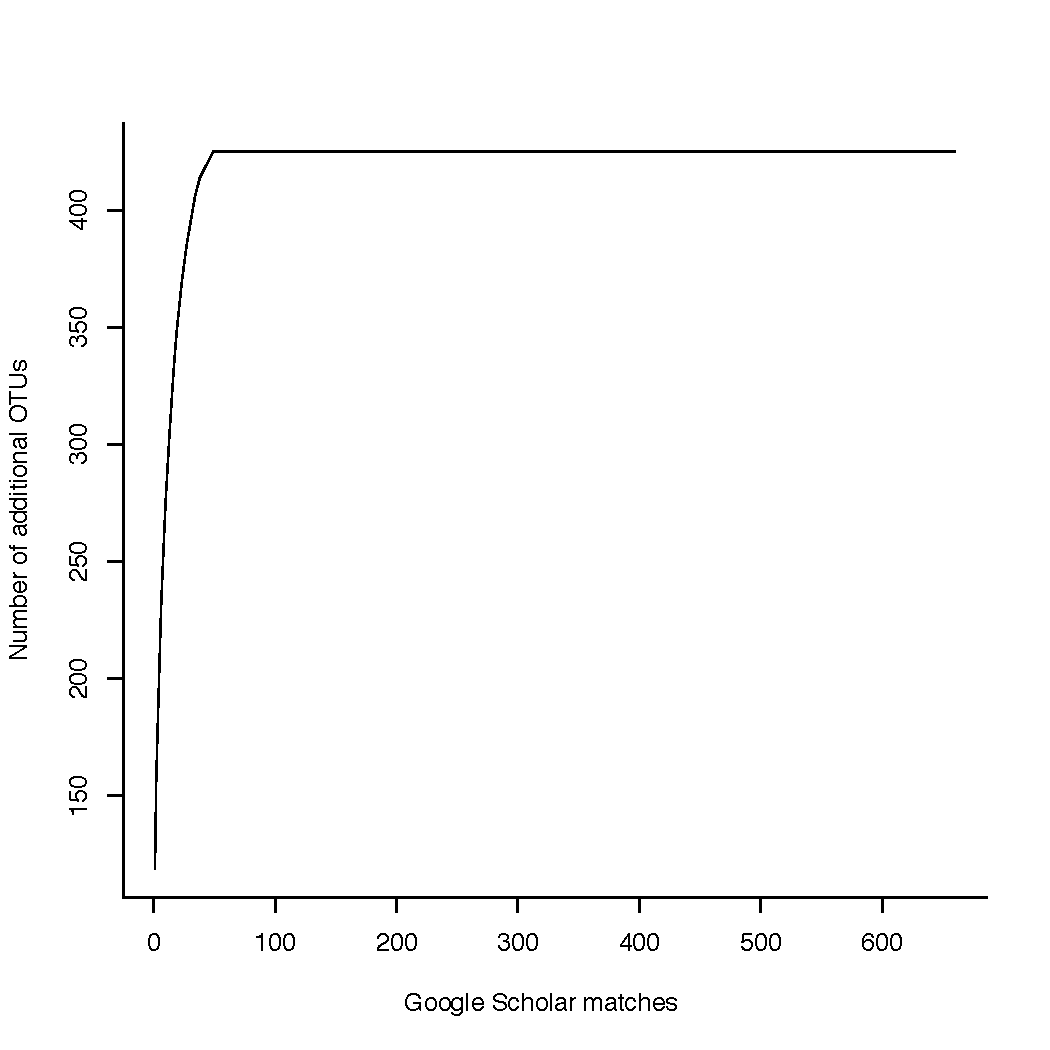
\includegraphics[width=1\textwidth]{Supplementary/Supp_figure_google_searches.pdf}
\caption{Google searches additional OTUs rarefaction curve. The x axis represent the number of google scholar matches (papers, books or abstracts) and the y axis represents the cumulative number of additional living OTUs per google scholar match.}
\label{Supp_figure_google_searches}
\end{figure}


\subsection{Wrong Bionmial names and typos}
I fixed the wrong bionomial names format (e.g. H. sapiens) into the correct ones (e.g. Homo sapiens) manually using the abreviation list in the concerned publications. We then applied our taxonomic matching algorithm to classify the OTUs as either living or fossil.

\begin{figure}[!htbp]
\centering
    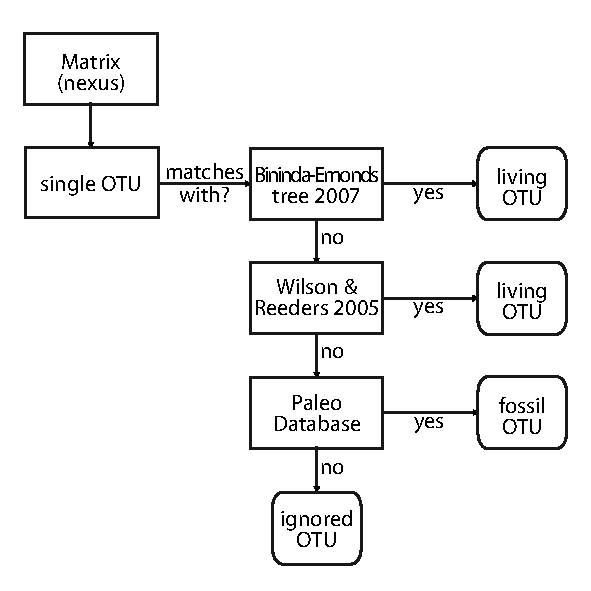
\includegraphics[width=1\textwidth]{Supplementary/Supp_figure_Taxonomic_algorithm.pdf}
\caption{Taxonomic matching algorithm used in this study. For each matrix, each operational taxonomic units (OTU) is matched with the super tree from Fritz 2009. If the OTU matches, then it is classified as living. Else it is matched with the Wilson \& Reeders 2005 taxonomy list. If the OTU matches, then it is classified as living. Else it is matched with the Paleo Database list of mammals. If the OTU matches, then it is classified as fossil. Else it is ignored.}
\label{Supp_figure_Taxonomic_algorithm}
\end{figure}

\bibliographystyle{vancouver}
\bibliography{Supp_References}


\section{Data structure}
%Tables
%Figures

\section{Supplementary results}



%END
\end{document}
